
\begin{center}
\Huge
Aflevering 3
\end{center}

\section*{Opgave 1}
\stepcounter{section}
To funktioner $f$ og $g$ er givet ved henholdsvist
\begin{align*}
f(x) = 2\sqrt{2x} \textnormal{ og } g(x) = e^{x/2}.
\end{align*}
\begin{enumerate}[label=\roman*)]
\item Bestem den afledede af $f$ og $g$ og bestem $f'(2)\cdot g'(2)$.
\item Bestem det ubestemte integrale 
\begin{align*}
G(x) = \int g(x) \intd x.
\end{align*}
\item Bestem funktionen $h(x) = f(G(x))$.
\item Bestem ligningen for tangenten af $h(x)$ i punktet $(3,h(3))$.
\end{enumerate}

\section*{Opgave 2}
\stepcounter{section}
Vi ønsker at bygge en aflang flyhangar. Den skal have et rumfang på $26000$m$^3$, og den skal være dobbelt så lang som bred, og den skal have en åbning foran. En skitse af hangaren kan ses på Fig. \ref{fig:hangar}. Der skal ikke være bund i hangaren. 
\begin{figure}[H]
\centering
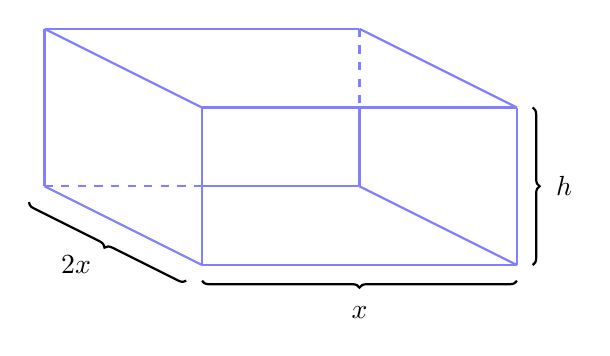
\begin{tikzpicture}

\draw[color = blue!50, thick] (0,0) to (4,0);
\draw[color = blue!50, thick] (0,2) to (4,2);
\draw[color =blue!50, thick] (4,2) to (4,0);
\draw[color = blue!50, thick] (0,0) to (0,2);

\draw[color = blue!50, thick] (0,0) to (-2,1);
\draw[color = blue!50, thick] (0,2) to (-2,3);
\draw[color = blue!50, thick] (4,2) to (2,3);
\draw[color =blue!50, thick] (-2,3) to (2,3);
\draw[color =blue!50, thick] (-2,1) to (-2,3);
\draw[color =blue!50, thick] (4,0) to (2,1);

\draw[color = blue!50, thick,dashed] (-2,1) to (0,1);
\draw[color =blue!50, thick,dashed] (2,3) to (2,2);
\draw[color =blue!50, thick] (0,1) to (2,1);
\draw[color =blue!50, thick] (2,1) to (2,2);

\draw[decorate, decoration={brace,mirror},thick] (0,0-0.2) to (4,0-0.2); 
\draw[decorate, decoration={brace},thick] (0-0.2,0-0.2) to (-2-0.2,1-0.2); 
\draw[decorate, decoration={brace,mirror},thick] (4+0.2,0) to (4+0.2,2); 

\node at (2,-0.6) {$x$};
\node at (-1.6,0) {$2x$};
\node at (4.6,1) {$h$};
\end{tikzpicture}
\caption{Figur af hangar}
\label{fig:hangar}
\end{figure}
\begin{enumerate}[label=\roman*)]
\item Bestem et udtryk for rumfanget af hangaren
\item Bestem et udtryk for overfladearealet af hangaren. Husk, at der ikke skal være bund i hangaren. Der skal heller ikke være nogen side i hangaren i den side, der vender mod læseren på Fig. \ref{fig:hangar}.
\item Udnyt, at rumfanget af hangaren skal være $26000$m$^3$ til at bestemme et udtryk for $h$.
\item Brug dette udtryk for $h$ til at finde et udtryk for overfladearealet, der kun afhænger af $x$. 
\item Find det $x$, der gør overfladearealet af hangaren så småt som muligt. Hvad er det optimale overfladeareal?
\end{enumerate}

\section*{Opgave 3}
\stepcounter{section}
Tabel \ref{tab:tab1} beskriver antallet af bakterier $N$ i en opløsning efter tid $t$. Enheden for $N$ er mio. bakterier og $t$ er tid i timer. 
\begin{table}[H]
\centering
\begin{tabular}{c|c|c|c|c|c|c|c|c|c|c|c|c}
$t$ & 0 & 1 & 2 & 3 & 4 & 5 & 6 & 7&8&9&10&11\\ \hline
$N(t)$ & 2,8 & 3 & 3 & 3,4 & 3,7 & 4,2 & 4,7 & 4,8 & 5,8 & 6,4 & 7,5 & 9,2
\end{tabular}
\caption{Bakterievækst}
\label{tab:tab1}
\end{table}
\begin{enumerate}
\item Bestem den eksponentialfunktion $\hat{N}$, der bedst beskriver datasættet Tabel \ref{tab:tab1}. 
\item Bestem $\hat{N}'(x)$, og bestem derefter $\hat{N}'(24)$. Hvad er betydningen af tallet $\hat{N}'(24)$?
\item Omskriv $\hat{N}(x)$ til formen $be^{kx}$, og bestem derefter fordoblingskonstanten for $\hat{N}$. Hvad fortæller fordoblingskonstanten os?
\item Hvor mange bakterier er der i følge modellen $\hat{N}$ efter en uge, og med hvor mange bakterier vokser bakterierne per time efter en uge i følge modellen? Bliver modellen ved med at kunne beskrive væksten af bakterierne?
\end{enumerate}

\section*{Opgave 4}
\stepcounter{section}
Betragt funktionerne $f$ og $g$ givet ved
\begin{align*}
f(x) = \frac{1}{x} \textnormal{ og } g(x) = 3x^3+2x.
\end{align*}
\begin{enumerate}[label=\roman*)]
\item Bestem integralerne 
\begin{align*}
\int f(x) \intd x \textnormal{ og } \int g(x) \intd x.
\end{align*}
\item Bestem det ubestemte integral
\begin{align*}
H(x) = 10f(x) \intd x - \frac{1}{2}\int g(x) \intd x.
\end{align*}
\item Bestem nu $H$, så grafen for $H$ går gennem punktet $(1,1)$.
\end{enumerate}